\section{Experimental setup}
\subsection{Method}
To measure the absorption spectra of stainless steel and natural iron, we irradiate the samples with the $14.4keV$ $\gamma$-radiation emitted by a radioactive source. To vary the frequency a motor is used to move the absorber relative to the source (Doppler shift see  \ref{eq:diffdopplershift}). By repeating this measurement for different absorber velocities a spectrum is recorded.\\
\subsection{Setup}
\begin{figure}[hbt]
\centering
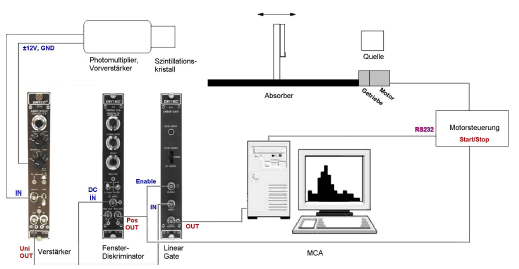
\includegraphics[width=1.0\linewidth]{graphics/Aufbau}
\caption[Setup overview ]{Overview of the experimental setup}
\label{fig:Aufbau}
\end{figure}

The setup consists of the $\gamma$ source, the absorber on a track, the motor used to move the absorber at constant speeds relative to the source and as the photon detector a scintillator is used. The light signal of the scintillator turned into an electric signal by a photomultiplier. This signal is amplified and shaped in the amplifier. The amplifier has two exits, one of which is connected to a single channel analyzer (SCA). If the signal pulse is within an adjustable window the SCA sends a standardized signal and enables the linear gate, which is also connected to the amplifier via a delay to ensure simultaneity of the signals. If the linear gate is enabled when it receives a signal from the amplifier it transmits the amplifier signal to the multichannel analyzer (MCA), which is read out with a Computer. The second output of the SCA is connected to a counter, which also can be read out with the Computer.

\subsection{The source Co-57}
\isotope[57]{Co} decays via electron capture with a branching ratio of $99.8 \%$ and a half life of 270d into an iron in an excited state $\isotope[57]{Fe^*}$. This state decays with a half life of 9ns an branching ratio of $88\%$ into the $14.4keV$ excited state which finally decays to the ground state (Branching ratio for $\gamma-decay$ is $10\%$) \ref{fig:principles:Zerfallsschema2}. 
\begin{figure}[hbt]
	\centering
	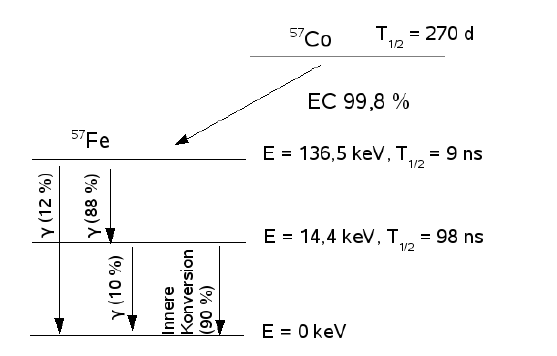
\includegraphics[width=0.5\linewidth]{graphics/Zerfallsschema2}
	\caption[Co-57 decay]{decay series of Cobalt-57}
	\label{fig:principles:Zerfallsschema2}
\end{figure}
\subsection{Procedure}
\subsubsection{MCA calibration}
To calibrate the MCA the spectra of Cu, Rb, Mo, Ag, Ba, and Tb are measured for 300s each. For the Cu no peak
\subsubsection{background measurement}
